\section{Zielsetzung}
Im diesem Versuch wird die Funktionsweise eines Geiger-Müller-Zählrohrs untersucht.

\section{Theorie}
\subsection{Aufbau}
Der Aufbau eines Geiger-Müller-Zählrohrs ist in Abbildung \ref{abb:1} dargestellt. Hauptsächlich besteht dieses aus einem mit Gas gefüllten Hohlzylinder,
welcher als Kathode dient, und einem Anodendraht in der Mitte. Das Gas ist meist ein Gemisch aus Argon und Ethylalkohol. Wird nun eine Spannung an das
Geiger-Müller-Zählrohr angelegt ensteht ein radialsymmetrisches elektrisches Feld im Inneren des Rohrs, welches beschrieben wird durch
\begin{equation*}
  E(r) = \frac{U}{\symup{ln}(r_k/r_a)} \cdot \frac{1}{r} \ ,
\end{equation*}
wobei $r_k$ den Radius des Hohlzylinders, $r_a$ den Radius des Anodendrahtes und $U$ die anliegende Spannung beschreibt. Da mit dem Geiger-Müller-Zählrohr
vor allem \alpha- und \beta-Strahlung nachgwiesen werden kann und diese aber von dem Hohlzylinder absorbiert werden würden, ist das Eintrittsfenster aus
Mylar-Folie, welches sogar auch \alpha-Strahlung hindurch lässt.
\begin{figure}
  \centering
  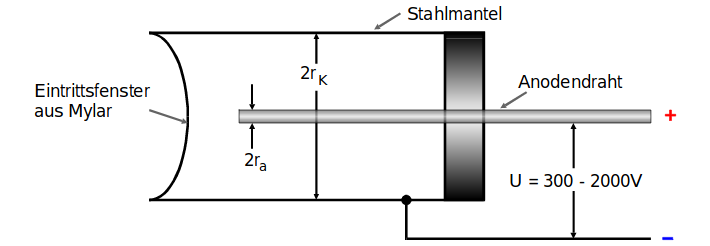
\includegraphics[scale=0.5]{a.png}
  \caption{Aufbau eines Geier-Müller-Zählrohrs. \cite{Q1}}
  \label{abb:1}
\end{figure}

\subsection{Funktionsweise}
In einem Geiger-Müller-Zählrohr kann \alpha- und \beta-Strahlung zu fast \SI{100}{\percent} nachgewiesen werden, \gamma-Stahlung hingegen ist zu hochenergetisch, hier kann nur
Strahlung mit hohen Intensitäten nachgewiesen werden, da die Wechselwirkung mit Materie hier relativ gering ist.
Gelangt nun ein geladenens Teilchen in das Volumen des Geiger-Müller-Zählrohrs, führt dies dazu, dass ein Teilchen aus dem Gas ionisiert wird. Die
Ionisation führt dazu, dass ein Kation und ein Elektron entstehen: Das Elektron wird durch das elektrische Feld in Richtung des Anodendrahtes beschleunigt
und dort absorbiert. Der daraus entstehende Elektrische Impuls wird durch einen Kondensator ausgekoppelt und verstärkt, sodass ein Zähler die Impulse messen kann.
Das Kation hingegen wird in Richtung des Kathodenzylinders beschleunigt und eigentlich im Kathodenmaterial absorbiert. Hierbei ist
aber zu beachten, dass das Kation eine hohe Energie hat und somit aus dem Kathodenmaterial weitere Elektronen herauslösen kann, diese werden
als \textbf{Sekundärelektronen} bezeichnet. Würde man diesen Effekt nicht verhindern, würden diese Elektronen zu einem weiteren Ausschlag des Geiger-Müller-Zählrohrs
führen. Dieser Effekt kann aber durch Hinzugabe von Ethylalkoholgas verhindert werden, denn die Kationen werden von diesen Atomen absorbiert und regen diese
zu Schwingungen an. Somit gelangen die Kationen nicht mehr bis zu dem Kathodenmaterial und können auch somit keine Sekundärelektronen mehr herauslösen.
Da die Energie des eintreffenden, geladenen Teilchens viel höher ist, als die Ionisierungsenergie, können mehrere Ionisationen gleichzeitig stattfinden.
Der weitere Verlauf nach der Ionisierung hängt stark von der angelegten Spannung ab:
\begin{itemize}
  \item Für niedrige Spannungen (siehe Abbildung \ref{abb:2}, Bereich I) ist die Wahrscheinlichkeit einer \textbf{Rekombination} sehr hoch. Durch die Rekombination
  wird die Ionisation rückgängig gemacht. Es enstehen in diesem Bereich also nur sehr geringe, kaum messbare Ströme.
  \item Im Proportionalitätsbereich (siehe Abbildung \ref{abb:2}), Bereich II und III) regt die oben beschriebene Ionisation weiter Ionisationen an, indem
  das ionisierte Elektron durch das elektrische Feld in Richtung des Anodendrahtes beschleunigt wird. Hierbei gewinnt es so viel Energie, dass
  es ein weiteres Atom zu Ionisierung anregen kann. So ensteht schnell eine \textbf{Elektronenlawine}. Wichtig in diesem Bereich ist außderdem, dass die gemessenen
  elektrischen Impulse proportinal zu der \textbf{Energie} und der \textbf{Intensität} der eindringenden Strahlung ist.
  \item In dem Spannungsbereich des Geiger-Müller-Zählrohrs (siehe Abbildung \ref{abb:2}, Bereich IV) kommt zu der Elektronenlawine noch ein weiter Effekt hinzu:
  Bei der Elektronenlawine enstehen nicht nur eine große Anzahl an Elektronen, sondern für hohe Spannungen auch \textbf{UV-Photonen}. Diese können, aufgrund ihrer
  neutralen Ladung, auch senkrecht oder entgegengesetzt der Feldlinien in dem Zylinderkondensator bewegen und somit weitere Atome und somit Elektronenlawinen anregen.
  In diesem sogenannten \textbf{Auslösebereich} ist der gemessene elektrische Impuls jetzt nurnoch von der \textbf{Intensität} abhängig und es kann keine Aussage mehr
  über die Energie der Strahlung getroffen werden.
  \item Überschreitet man den Auslösebereich und erhöht die Spannung weiter, so wird durch eine einzelne Ionisation eine Dauergasentladung enzündet und
  das Geiger-Müller-Zählrohr wird durch daraus entstehende zu hohe Stromdichten zerstört. Dies wird der Bereich der \textbf{selbständigen Gasentladung} genannt.
\end{itemize}
\begin{figure}
  \centering
  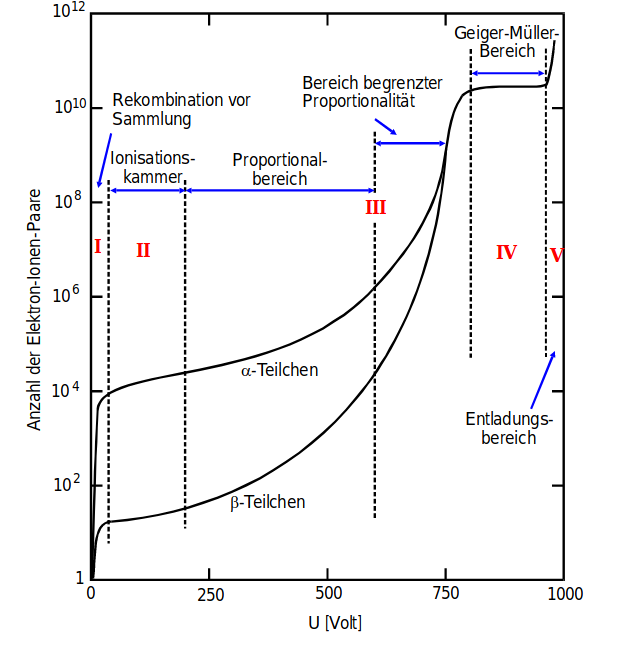
\includegraphics[scale=0.4]{b.png}
  \caption{Anzahl Elektronen in Abhängigkeit der Spannung. \cite{Q1}}
  \label{abb:2}
\end{figure}

\subsection{Totzeit und Erholungszeit}
Im Gegensatz zu Elektronen, die sich durch ihre geringe Masse relativ schnell zum Anodendraht bewegen, werden die positiv geladenen Kerne durch ihre größere Masse
langsamer beschleunigt und benötigen für die Zeit bis zur Kathode länger. Da diese nicht instantan zum Kathodenmaterial gelangen, bildet sich für eine kurze Zeit eine
positive Raumladung, auch \textbf{Ionenschlauch} genannt, welche sich dem elektrischen Feld entgegensetzt. Das führt dazu, dass in dem Bereich um den Anodendraht
keine Ionisationen mehr möglich sind. Also auch wenn in diesem Zeitraum ein weiteres geladenenes Teilchen in das Zählrohrvolumen eintritt, kann dies nicht detektiert werden.
Man definiert also eine Zeit $T$, in der es nach einer Detektion nicht möglich ist, weitere Teilchen zu detektieren, die sogenannte \textbf{Totzeit}.
Nach solch einer Ionisationslawine und der Totzeit müssen die Ionen zunächst wieder vollständig neutralisiert werden, damit das elektrische Feld nicht mehr durch
Ionen gestört werden kann. Diese Zeit wird \textbf{Erholungszeit} genannt.
Diese beiden charakteristischen Zeiten können an einem OSzilloskop durch Darstellung des elektrischen Impulses abgelesen werden. Außerdem gibt es für die Messung der
Totzeit noch die \textbf{Zwei-Quellen-Methode}: Hierbei wird in einem Zeitintervall eine Messung mit der Quelle $Q_1$ durchgeführt, darauf folgend eine Messung im selben
Zeitintervall mit der Quelle $Q_1$ und $Q_2$ und zuletzt eine Messung mit der Quelle $Q_2$. Hierbei sollten sich die jeweiligen Quellen zu den Messungen an der selben
Stelle befinden. Das Ergebnis dieser Messungen wird hervorbringen, dass gilt
\begin{equation*}
  N_{\symup{1+2}} < N_1 + N_2
\end{equation*}
wobei $N$ jeweils die Anzahl der Counts ist.
Aus dieser Relation kann man näherungsweise die Totzeit $T$ bestimmen durch
\begin{equation}
  \label{eq:Totzeit}
  T \approx \frac{N_1+N_2-N_{\symup{1+2}}}{2N_1N_2}
\end{equation}
Die Totzeit und die Erholungszeit sind in Abbildung \ref{abb:3} dargestellt.
\begin{figure}
  \centering
  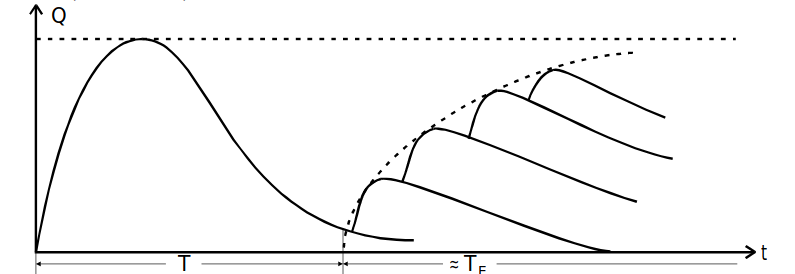
\includegraphics[scale=0.4]{c.png}
  \caption{Totzeit und Erholungszeit eines Geiger-Müller-Zählrohrs. \cite{Q1}}
  \label{abb:3}
\end{figure}


\subsection{Charakteristik eines Zählrohrs}
Die Charakteristik eines Geiger-Müller-Zählrohr wird bei konstanter Intensität aufgenommen, hierzu wird die Spannung gegen die erfasste Teilchenanzahl aufgetragen.
Solch eine Charakteristik ist in Abbildung \ref{abb:4} zu sehen.
\begin{figure}
  \centering
  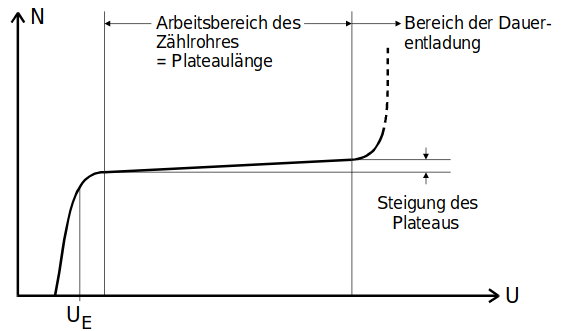
\includegraphics[scale=0.5]{d.png}
  \caption{Charakteristik eines Geiger-Müller-Zählrohrs. \cite{Q1}}
  \label{abb:4}
\end{figure}
Etwa nach der Spannung $U_E$ setzt der Auslösebereich ein, hier beginnt bei der Charakteristik das Plateau. Dieses Plateau hat idealerweise keine Steigung, dies kann aber
aufgrund von Nachentladungen nicht erreicht werden. Je geringer die Stigung und je länger das Plateau, desto höher ist die Qualität des Geiger-Müller-Zählrohrs.
Nach dem Plateau schließt sich der Bereich der Dauerentladung an, hierbei kann das Zählrohr für hohe Spannungen zerstört werden.

\subsection{Messung der pro Teilchen vom Zählrohr freigesetzten Ladungsmenge}
Durch den mittleren Zählrohrstrom $\bar{I}$ kann außerdem die Ladung $\Delta Q$ berechnet werden, hierzu werden die Definitionen
\begin{align*}
  \bar{I} &= \int_0^{\tau} \frac{U(t)}{R} \symup{d}t \\
  \bar{I} &= \frac{\symup \Delta Q}{\symup \Delta t} \, Z
\end{align*}
gleichgesetzt, wobei $U(t)$ die Spannung, $R$ der Widerstand, $\symup \Delta t$ das Zeitintervall, $\symup \Delta Q$ die in dem Zeitintervall $\symup \Delta t$
gemessene Ladung und $Z$ die Anzahl der registrierten Teilchen beschreibt.

\section{Durchführung}
Der Versuch wird nach Abbildung \ref{abb:5} aufgebaut. Zur Messung wird ein \beta-Stahler vor dem Geiger-Müller-Zählrohr platziert.

\begin{figure}
  \centering
  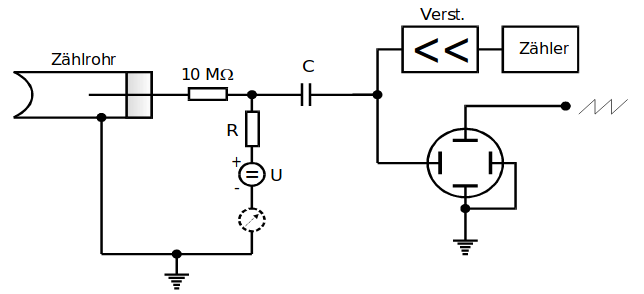
\includegraphics[scale=0.5]{e.png}
  \caption{Versuchsaufbau. \cite{Q1}}
  \label{abb:5}
\end{figure}

Zur Messung der Charakteristik des Geiger-Müller-Zählrohrs werden die Counts in Abhängigkeit der Spannung gemessen. Hierbei wird ein Bereich von
\SI{300}{\volt} bis \SI{700}{\volt} in \SI{10}{\volt}-Schritten abgetastet und die jeweiligen Counts in einer Zeit von $\Delta t = \SI{60}{\second}$ gemessen.

Im zweiten Teil des Versuch soll die Totzeit $T$ und die Erholungszeit $T_{\symup{er}}$ gemessen werden. Hierzu werden die elektrischen Impulse auf dem Oszilloskop
sichtbar gemacht und durch den Trigger an einer Stelle zum Stehen gebracht. Nun wird die Totzeit an abgelesen, indem man die Breite des Impulses abließt.
Die Erholungszeit kann dadurch bestimmt werden, dass man die Zeit zwischen dem Ende des Hauptimpulses und dem Anfang des nächsten Impulses misst, welcher
genauso hoch sein muss, wie der Hauptimpuls. An der Stelle haben sich die Ionen wieder vollständig neutralisiert und es kann ein neuer Impuls gemessen werden.
Diese Messungen werden für 5 verschiedene Spannungen im bereich des Plateaus durchgeführt.

Zur genaueren Messung der Totzeit wird außerdem die Zwei-Quellen-Methode einmal durchgeführt, indem je beide Quellen einzeln und einmal beide Quellen zusammen
in einem Zeitintervall von \SI{60}{\second} gemessen werden. Die Spannung beträgt hierbei \SI{550}{\volt}.

Zuletzt soll die Abhängigkeit der Ladung von der Spannung bestimmt werden, hierzu werden für mindestens 5 verschiedene Spannungen zwischen \SI{300}{\volt} und
\SI{700}{\volt} die Counts und die Stromstärke gemessen.
